\documentclass[a4paper,10pt,oneside]{article}
\usepackage{graphicx}
\usepackage{color}
\usepackage{url}
\usepackage{subfigure}
\usepackage[utf8]{inputenc}
\usepackage[T1]{fontenc}
\usepackage{tgpagella}
%\usepackage[scale=0.9]{tgcursor}
%\usepackage[scale=0.9]{tgheros}
\usepackage{xstring}

\newcommand{\myscale}{0.74}
\newcommand{\vect}[1]{\boldsymbol{#1}}
\newcommand{\code}[1]{\texttt{\StrSubstitute{#1}{.}{.\.}}}
\def\.{\discretionary{}{}{}}
\newcommand{\jmodule}[1]{\texttt{\textit{#1}}}

\setlength{\hoffset}{-1in} %left margin will be 0, as hoffset is by default 1inch
\setlength{\voffset}{-1in} %analogous voffset
\setlength{\oddsidemargin}{1.5cm}
\setlength{\evensidemargin}{1.5cm}
\setlength{\topmargin}{1.5cm}
\setlength{\textheight}{24cm}
\setlength{\textwidth}{18cm}

\def\mftitle{jInfer ProjectType Module Description}
\def\mfauthor{Michal Klempa, Mário Mikula, Robert Smetana, Michal Švirec, Matej Vitásek}
\def\mfadvisor{RNDr. Irena Mlýnková, Ph.D., Martin Nečaský, Ph.D.}
\def\mfplacedate{Praha, 2011}
\title{\bf\mftitle}
\author{\mfauthor \\ Advisors: \mfadvisor}
\date{\mfplacedate}

\ifx\pdfoutput\undefined\relax\else\pdfinfo{ /Title (\mftitle) /Author (\mfauthor) /Creator (PDFLaTeX) } \fi

\begin{document}
\maketitle
\noindent Target audience: developers willing to extend jInfer, specifically extend jInfer project structure.

\noindent \begin{tabular}{|l|l|} \hline
Responsible developer: & Michal Švirec \\ \hline
Required tokens:       & cz.cuni.mff.ksi.jinfer.base.interfaces.inference.IGGenerator \\
 & cz.cuni.mff.ksi.jinfer.base.interfaces.inference.SchemaGenerator \\
 & cz.cuni.mff.ksi.jinfer.base.interfaces.inference.Simplifier \\
 & org.openide.windows.IOProvider \\ \hline
Provided tokens:       & none \\ \hline
Module dependencies:   & Base \\
	& Runner \\ \hline
Public packages:       & cz.cuni.mff.ksi.jinfer.projecttype.actions \\ \hline
\end{tabular}

\section{Introduction}

\jmodule{ProjectType} is the module responsible for creation of NBP project type which groups input/output files that belongs to one specific inference. Each jInfer project also allows user to set properties specific for inference.

\section{Structure}

Structure of \jmodule{ProjectType} can be divided into following five main parts.
\begin{itemize}
	\item Base classes - Classes providing main functionality like creation of project, defining operations like move, delete, copy etc. All the base classes are contained in the \code{cz.cuni.mff.ksi.jinfer.projecttype} package.
	\item Visualization classes - These classes create tree structure of project in NBP Projects view and are contained in the \code{cz.cuni.mff.ksi.jinfer.projecttype.nodes}
	\item Actions - Classes from \code{cz.cuni.mff.ksi.jinfer.projecttype.actions} package that provides actions allowing adding, removing input files into project, or running the project.
	\item Properties - Classes responsible for creation of project properties window with properties category tree. These are situated in  \code{cz.cuni.mff.ksi.jinfer.projecttype.properties} package.
	\item Project wizard - Classes representing creation of project through new project wizard from  \code{cz.cuni.mff.ksi.jinfer.projecttype.sample} package.
\end{itemize}

\subsection{Base classes}

\begin{figure}
	\centering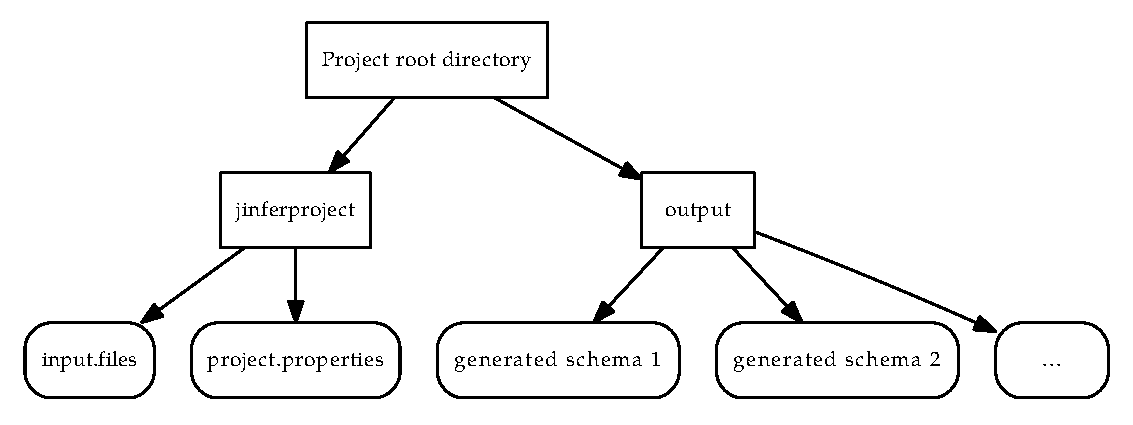
\includegraphics[scale=\myscale]{project_dir_structure}
	\caption{Project directory structure} \label{dir-structure}
\end{figure}

This section describes classes needed for creation of the jInfer project and correct integration into NBP. With each project created in jInfer is also created specific directory structure on filesystem that describes jInfer project. This structure is described in figure \ref{dir-structure}, where rectangles represent folders and rounded rectangles files.\\

Main two classes representing jInfer project type are \code{JInferProjectFactory} and \code{JInferProject}. \code{JInferProjectFactory} is a factory classes responsible for creation of jInfer project from disk directory and \code{JinferProject} is represent jInfer project in NBP.


\subsection{Visualization classes}

\subsection{Actions}

\subsection{Properties}

\subsection{Project wizard}

\subsection{Preferences}


\nocite{*}
\newpage
\bibliographystyle{alpha}
\bibliography{literature}

\end{document}
